\newpage
\section{Возможные неисправности и методы их устранения}
\subsection{Оплата по эквайрингу не прошла, клиенту пришло SMS  о списании со счета суммы покупки.}
Если после попытки безналичной оплаты клиенту пришло SMS о списании денег со счета, а на кассе эквайринговый чек не распечатался выполнить следующее:

\begin{enumerate}	
	\item Позвонить в контактный центр сбербанка по тел. \textbf{8-800-350-01-23} и сообщив номер терминала
	(высвечивается на экране терминала в левом нижнем углу) выяснить прошла ли данная оплата от клиента.

	\item Если сбербанк подтвердил прохождение оплаты то позвонить в техподдержку для ручного проведения операции продажи и распечатки фискального чека.
	
	\item Если сбербанк НЕ подтвердил оплату от клиента предложить провести попытку оплаты еще раз или заплатить наличкой.
		
\end{enumerate}	

\subsection{Фискальный (товарный) чек не напечатан после нажатия кнопки «Оплата» (безнал)}
%\marginnote{\Date{Пт.}{13}{Июл.}{2018}}[-40pt]

\begin{itemize}	
	\item После окончания подбора товара в чек и НАЖАТИЯ КНОПКИ «Оплата» (на клавиатуре или на экране), после проведения безналичной оплаты, фискальный (товарный)  чек не распечатан на фискальном регистраторе (окно оплаты закрылось, но товар остался в табличной части).. 
	\begin{figure}[h]
		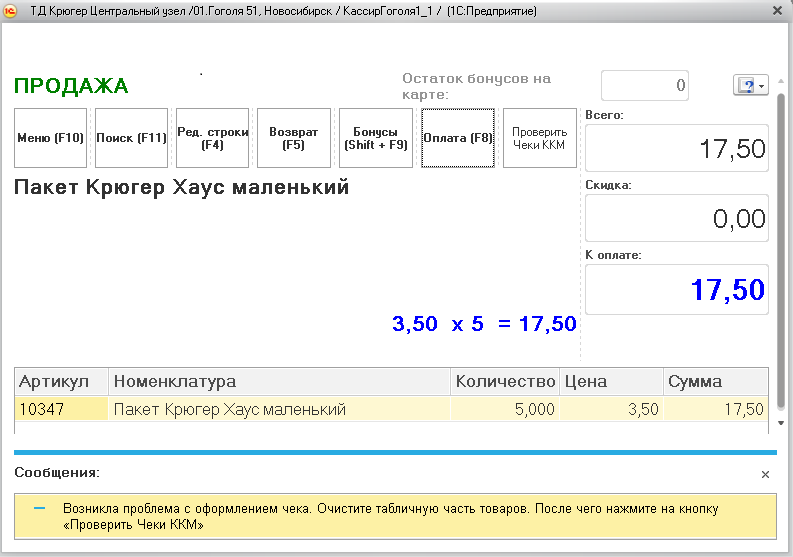
\includegraphics[width=0.6\textwidth]{6.png}
		\caption{Ошибка при оформлении чека}
		\label{ris:6.png}
	\end{figure}
	Нужно очистить табличную часть. (Удалить с экрана все товары) (Рис.~\ref{ris:6.png})	 
	При этом на экране станет активной кнопка <<Проверить Чеки ККМ>> (поз. 2) (Рис.~\ref{ris:7.jpg}).

	\begin{figure}[h]
		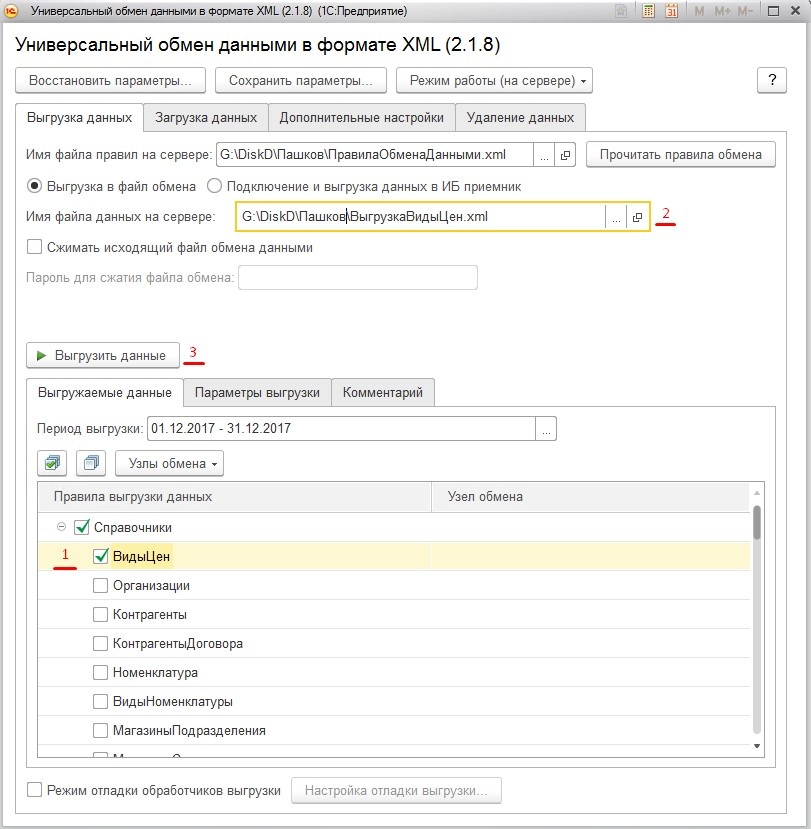
\includegraphics[width=0.5\textwidth]{7.jpg}
		\caption{Ошибка при оформлении чека}
		\label{ris:7.jpg}
	\end{figure}

	При нажатии на  кнопку <<Проверить Чеки ККМ>>  (Рис.~\ref{ris:7.jpg}) открывается форма списка проблемных чеков (Рис.~\ref{ris:8.png}).

	\textbf{ После прочтения сообщения в колонке <<Описание проблемы>>}  пробуем распечатать фискальный чек, нажав на кнопку (поз. 1) (Рис.~\ref{ris:8.png}).. При возникновении сообщения (поз. 2) (Рис.~\ref{ris:8.png}) требуется нажать на кнопку, (поз. 3) (Рис.~\ref{ris:8.png}). 
	
		\begin{figure}[H]
		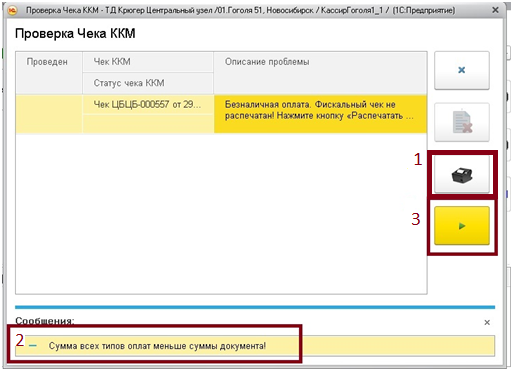
\includegraphics[width=0.7\textwidth]{8.png}
		\caption{Ошибка при оформлении чека}
		\label{ris:8.png}
	\end{figure}
	
	
	Откроется форма текущего проблемного чека (Рис.~\ref{ris:9.jpg}).
	

	\begin{figure}[H]
		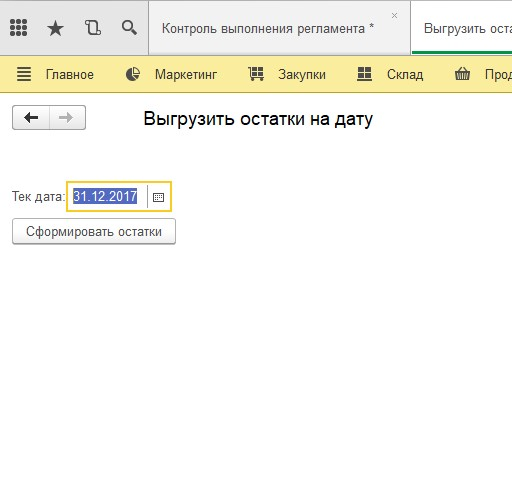
\includegraphics[width=0.7\textwidth]{9.jpg}
		\caption{Добавление оплаты}
		\label{ris:9.jpg}
	\end{figure}
	\par
%	\begin{figure}[h]
%		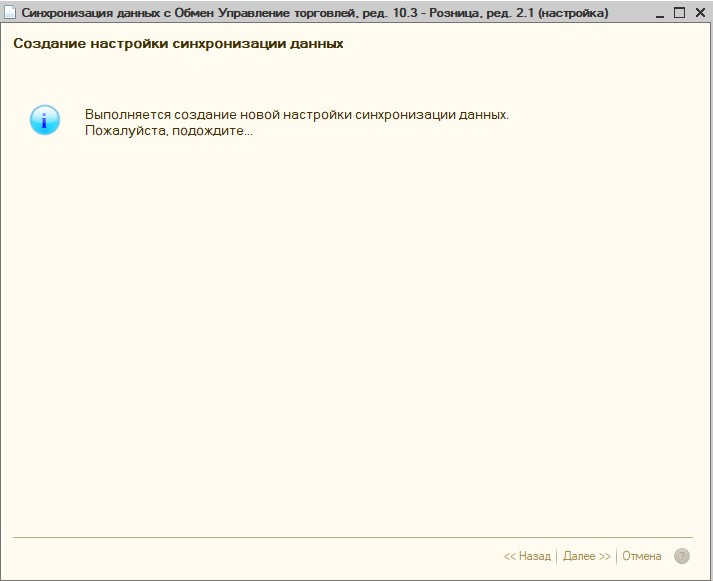
\includegraphics[width=0.5\textwidth]{10.jpg}
%		\caption{Форма чека}
%		\label{ris:10.jpg}
%	\end{figure}
\newpage
	Добавляем доступный вид оплаты. (Рис.~\ref{ris:11.jpg})

	\begin{figure}[H]
		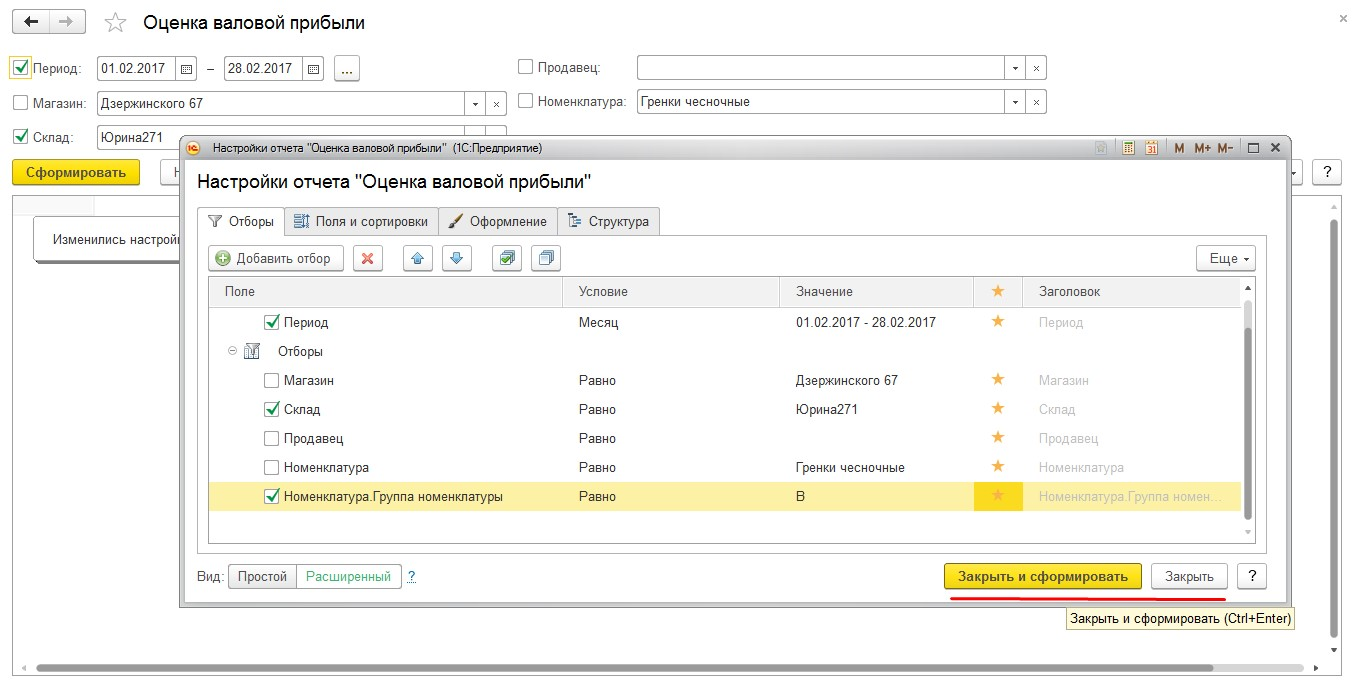
\includegraphics[width=0.5\textwidth]{11.jpg}
		\caption{Выбор формы оплаты}
		\label{ris:11.jpg}
	\end{figure}	

	\begin{figure}[h]
		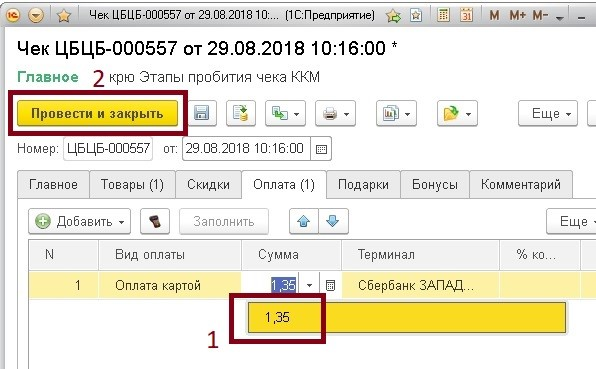
\includegraphics[width=0.5\textwidth]{12.jpg}
		\caption{Работа с чеком}
		\label{ris:12.jpg}
	\end{figure}	
	

	После  выбора формы оплаты выбрать требуемую сумму (поз. 1) (Рис.~\ref{ris:12.jpg}), провести и закрыть документ нажав кнопку <<Провести и закрыть>>. (поз. 2) (Рис.~\ref{ris:12.jpg}).

	Далее, после закрытия формы чека программа вернется в форму списка чеков (Рис.~\ref{ris:13.jpg}).
		\newpage
	\begin{figure}[H]
		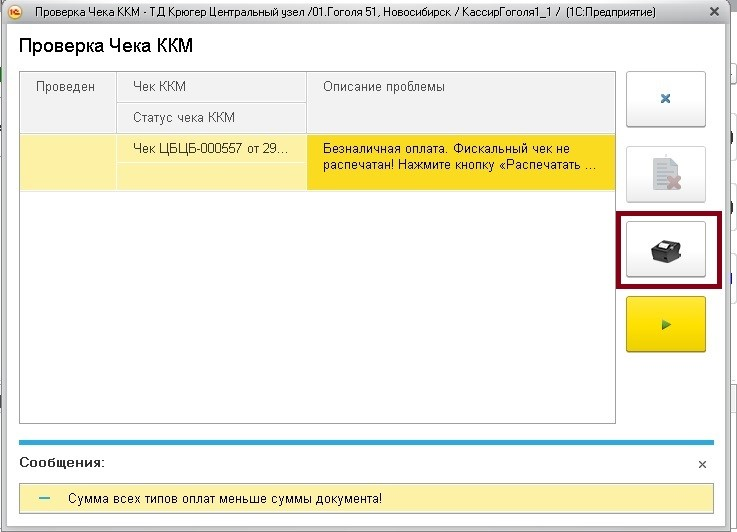
\includegraphics[width=0.7\textwidth]{13.jpg}
		\caption{Форма списка}
		\label{ris:13.jpg}
	\end{figure}	
	В открывшейся форме (Рис.~\ref{ris:13.jpg}) нажать на кнопку пробития чека. Чек будет распечатан на фискальном регистраторе
\subsection{Чек не вышел после нажатия <<Оплата>> (наличные)}	
	\item В случае наличной оплаты при печати фискального чека возникла проблема.
	Для удобного чтения сообщения можно нажать на кнопку (поз. 1) (Рис.~\ref{ris:14.jpg}) Тогда сообщение появится в окне. (Рис.~\ref{ris:14.jpg})
	
	\begin{figure}[H]
		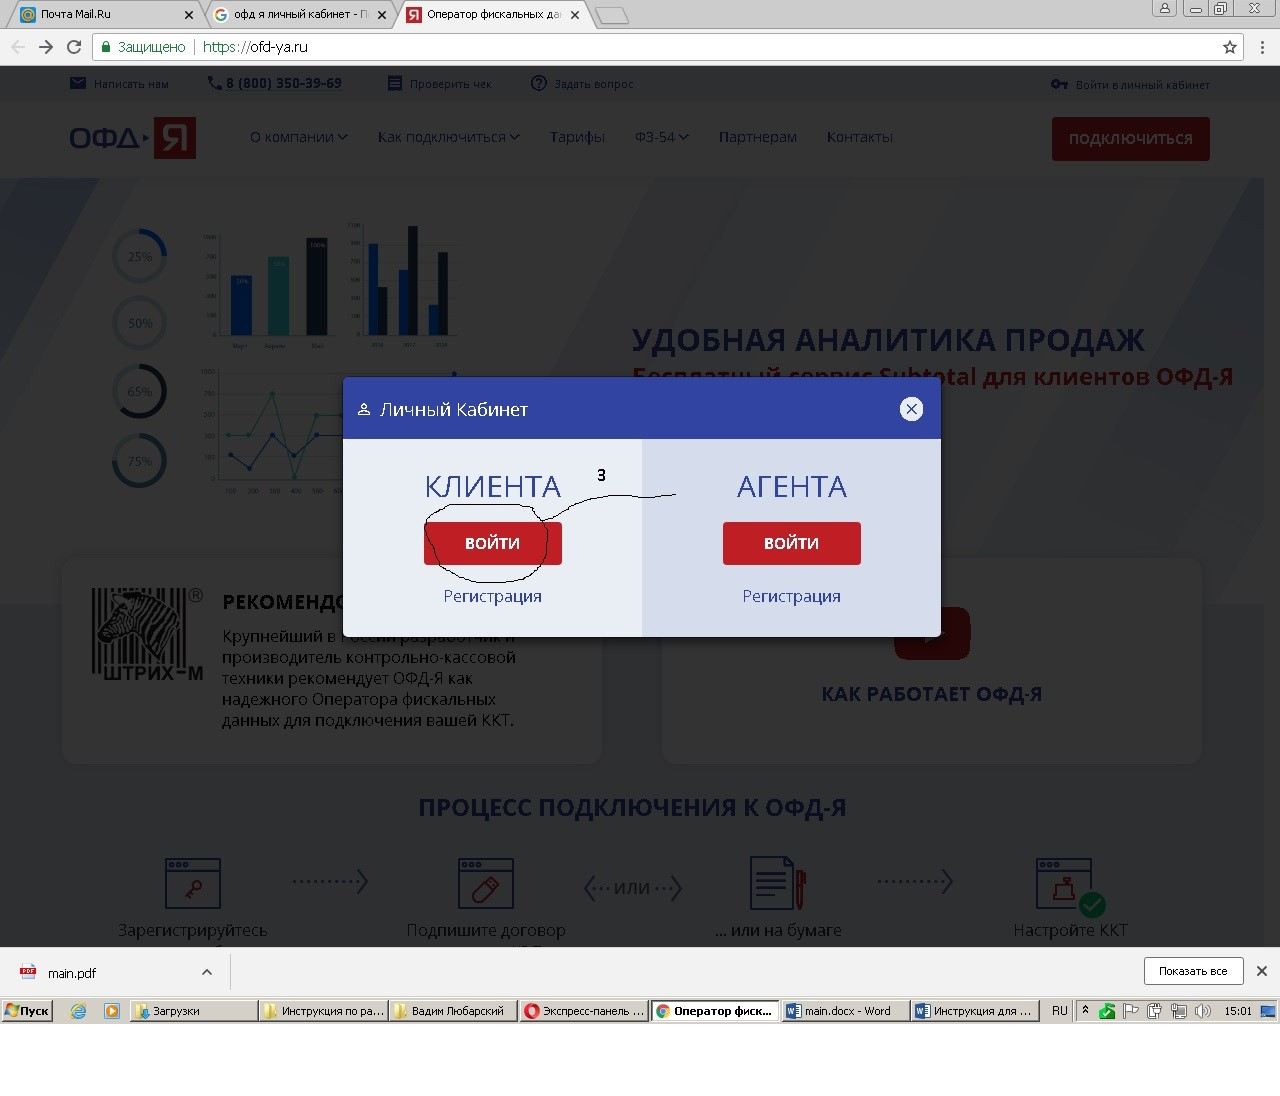
\includegraphics[width=0.7\textwidth]{14.jpg}
		\caption{Сообщения}
		\label{ris:14.jpg}
	\end{figure}		
	В подобных ситуациях после нажатия на кнопку печати фискального чека (поз. 2) (Рис.~\ref{ris:14.jpg}) выполнится проверка чека и ПРИ НЕОБХОДИМОСТИ он будет распечатан.
	
\end{itemize}
